@% Chapter 5

\chapter{Aplicação} % Main chapter title
\label{chap:Chapter5} % For referencing the chapter elsewhere, use \ref{chap:Chapter5} 

%----------------------------------------------------------------------------------------
\section{Sistema Desenvolvido}
O objetivo principal da parte prática da dissertação é não só recolher sinais e criar a sua função de ambiguidade, mas principalmente detetar um objeto estático e em movimento.
Para realizar estas tarefas foi utilizado um transmissor e recetor LimeSDR USB. As suas principais caraterísticas estão apresentadas na seguinte tabela e a sua documentação em \url{https://wiki.myriadrf.org/LimeSDR-USB}.\par

\begin{table}[h]
\centering
\begin{tabular}{@{}ccccc@{}}
\toprule
Caraterística       			 & Descrição                      \\ \midrule
\textit{RF Transreceiver}        & LMS7002M                       \\
\textit{Oscillator}    			 & Rakon RPT7050A @30.72$MHz$    \\
Banda de frequência              & 100$kHz$ - 3.8$GHz$            \\ 
Largura de banda máxima          & 61.44$MHz$                     \\ \bottomrule
\label{tab:limesdr}
\end{tabular}
\caption[Caraterísticas do LimeSDR USB]{Caraterísticas do LimeSDR USB}
\end{table}

Por forma a reduzir o ruído a alimentação é feita através dum \textit{power bank} de 20000$mAh$. Isto é conseguido com um cabo em "Y" que vem com o LimeSDR, que separa a entrada de dados da alimentação do equipamento.\par 
As duas antenas utilizada tanto para o canal de receção do sinal direto como do sinal refletido são antenas \textit{One for all} \textit{Yagi} de exterior para televisão, com $24dB$.\par 
Para a ligação entre o \textit{LimeSDR} e as antenas foram utilizados cabos coaxiais RG-58 com $1m$ de comprimento onde foram cravadas fichas SMA, como representado na figura \ref{fig:limec}.\par 
O repositório que contém as drivers que permitem trabalhar com o LimeSDR a partir do MATLAB pode ser acedido no \textit{github} do autor, \url{https://github.com/RakhDamir/LimeSDR-Matlab} feito inicialmente e disponibilizado no link \url{https://github.com/jocover/Simulink-MATLAB-LimeSDR} em Agosto de 2017 pelo autor Jocover, posteriormente adaptado e atualizado em Dezembro de 2019 pelo autor Damir Rakhimov para a versão do LimeSuite 19.04. Todos os passos de instalação e configuração do sistema encontram-se disponibilizados no seu \textit{github}.

\begin{figure}[h]
\centering
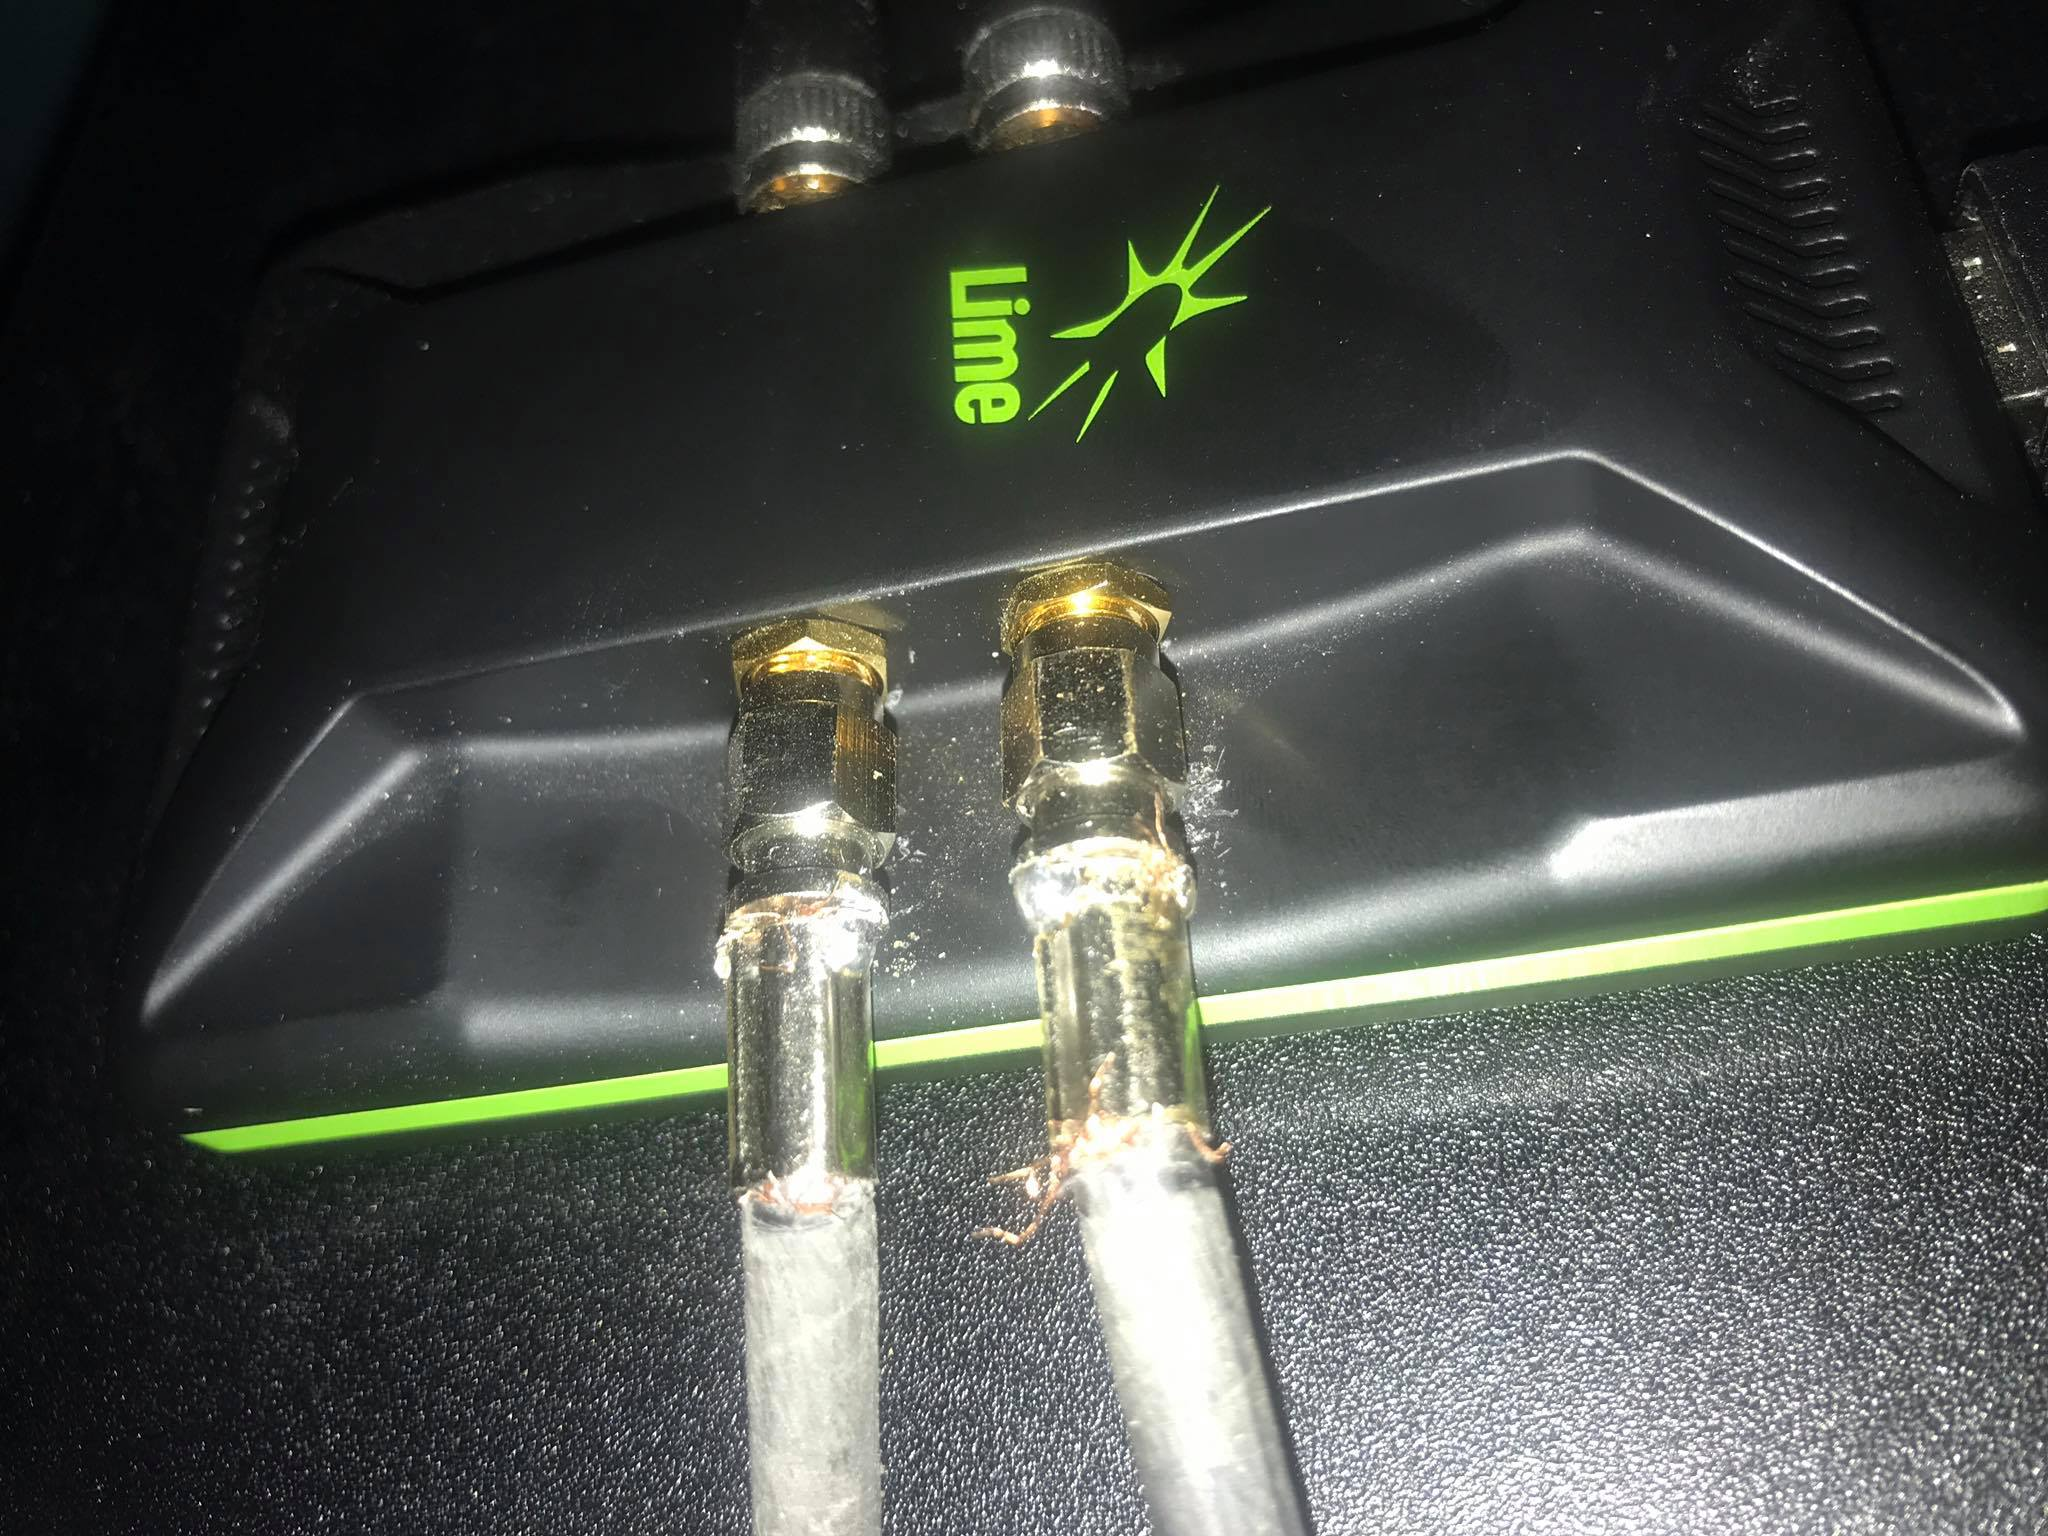
\includegraphics[scale=0.15]{chapters/ch5/assets/limec}
\caption[Entrada LimeSDR]{Entrada LimeSDR}
\label{fig:limec}
\end{figure}




\section{Resultados}


